{\color{gray}\hrule}
\begin{center}
\section{Understanding Obesity and T2D}
\textbf{Historical perspective and modern understanding of obesity and diabetes pathways}
\bigskip
\end{center}
{\color{gray}\hrule}
\begin{multicols}{2}
\subsection{Historical Perspective}
The understanding of obesity and Type 2 Diabetes (T2D) has evolved significantly over the past century. Early theories centered primarily on insulin resistance and beta-cell dysfunction as independent phenomena. Researchers initially viewed obesity as a simple imbalance between caloric intake and energy expenditure, while T2D was considered primarily a disorder of insulin production.

This simplified view, while providing a foundation for early treatments, failed to capture the complex interplay between adipose tissue, systemic inflammation, and metabolic regulation. The discovery of insulin in 1921 by Banting and Best marked a pivotal moment, but the intricate relationship between obesity and diabetes remained poorly understood for decades.

\subsection{Modern Understanding}
Current research reveals a more nuanced and interconnected pathway between obesity and T2D development. This process typically follows a predictable sequence:

\textbf{Early-Life Positive Energy Balance:} The pathway often begins in youth, where sustained excessive caloric intake relative to energy expenditure leads to increased fat storage. This early pattern establishes metabolic changes that can persist throughout life.

\textbf{Adipose Tissue Expansion and Metabolic Signals:} As fat mass expands, adipose tissue undergoes both quantitative and qualitative changes. The growing fat mass secretes increasing amounts of:
\begin{itemize}
    \item Pro-inflammatory cytokines
    \item Free fatty acids
    \item Adipokines that impair insulin signaling
\end{itemize}

\textbf{Insulin Resistance and Compensation:} In response to impaired insulin signaling, pancreatic $\beta$-cells increase insulin production to maintain normal glucose levels. This compensation leads to:
\begin{itemize}
    \item Chronic hyperinsulinemia
    \item Progressive insulin resistance
    \item Increased metabolic stress on $\beta$-cells
\end{itemize}

\textbf{$\beta$-Cell Stress and Dysfunction:} The sustained demand for high insulin production creates significant stress on $\beta$-cells, resulting in:
\begin{itemize}
    \item Reduced insulin secretion efficiency
    \item Progressive $\beta$-cell death
    \item Declining functional $\beta$-cell mass
\end{itemize}

\textbf{Progression to Youth-Onset T2D:} The combination of declining $\beta$-cell function and persistent insulin resistance ultimately leads to:
\begin{itemize}
    \item Inability to maintain normal glucose levels
    \item Development of prediabetes
    \item Eventually, full T2D onset
\end{itemize}

\end{multicols}

% Add figure here before pathway descriptions
\begin{figure}[h]
\centering
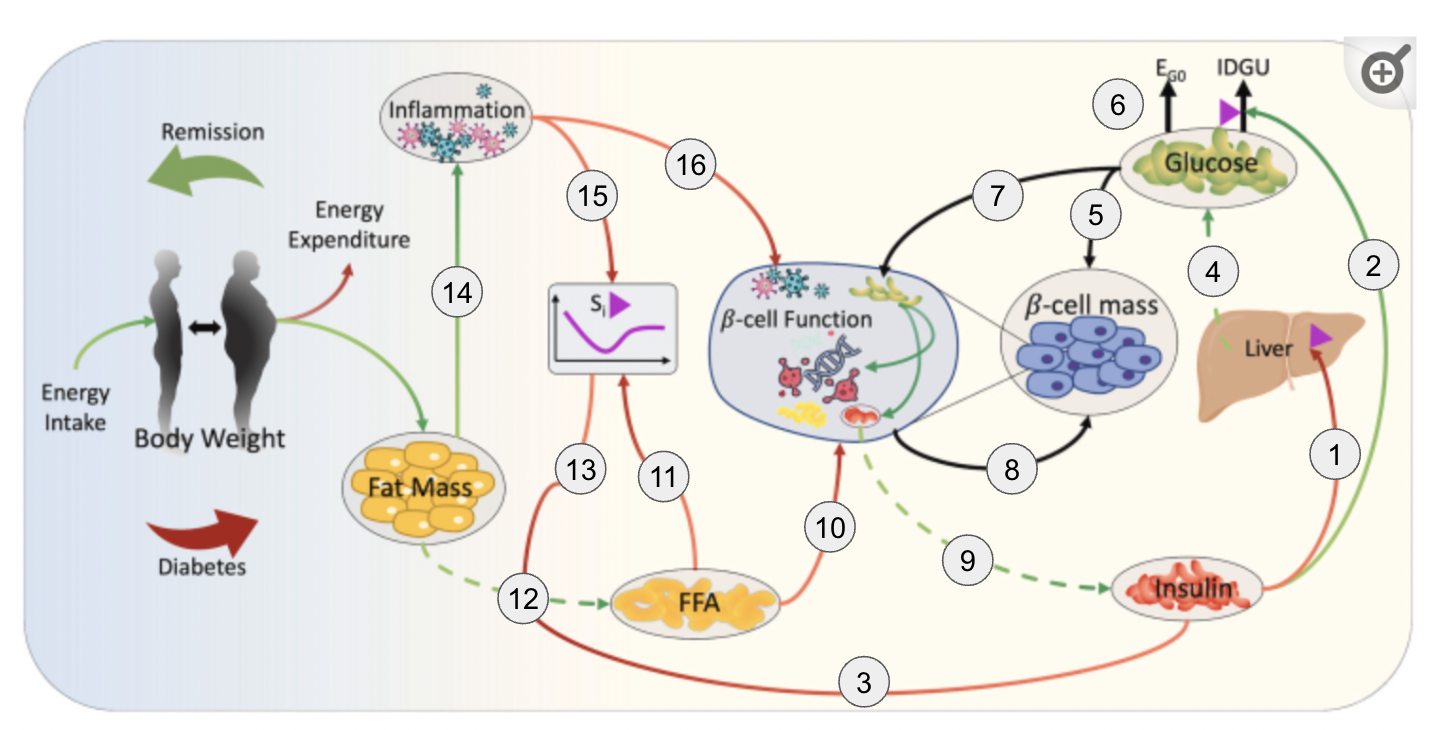
\includegraphics[width=0.8\textwidth]{images/obesity_and_t2d_diagram.png}
\caption{Interconnected pathways in obesity and T2D development. Numbers 1-16 correspond to specific metabolic interactions detailed below.}
\label{fig:pathways}
\end{figure}

\subsection{Pathway Integration}
Understanding these interconnected pathways is crucial for modern treatment approaches. The diagram above (Figure \ref{fig:pathways}) illustrates the complex feedback loops between these systems:

\begin{itemize}

    \item[\textbf{1.}] \textbf{Insulin to Liver:} (Insulin $\uparrow$) $\rightarrow$ (Hepatic Glucose Production $\downarrow$) \\
    High insulin levels increase hepatic insulin sensitivity, reducing the liver's glucose output. In the equation, $HGP = HGP_\text{bas} + \frac{\text{hepa\_max} \cdot (a_\text{hgp} + k_\text{gcg} \cdot gcg)}{(a_\text{hgp} + k_\text{gcg} \cdot gcg) + \text{hepa\_si} \cdot i}$, larger $i$ (insulin) in the denominator lowers HGP.
    
    \item[\textbf{2.}] \textbf{Insulin to Glucose:} (Insulin $\uparrow$) $\rightarrow$ (Peripheral Glucose Clearance $\uparrow$) \\
    Insulin enhances glucose uptake in peripheral tissues, increasing clearance. In the glucose balance, $dg = \text{gclamp} + HGP - (eg0 + sci \cdot si \cdot i)g$, a higher $i$ strengthens the removal term $(sci \cdot si \cdot i)g$.
    
    \item[\textbf{3.}] \textbf{Insulin to FFA:} (Insulin $\uparrow$) $\rightarrow$ (FFA Release $\downarrow$) \\
    Insulin suppresses lipolysis, reducing FFA release. The term $\frac{ksif^{aa}}{ksif^{aa}+(siff \cdot i)^{aa}}$ decreases as $i$ rises, cutting back on FFAs liberated into circulation.
    
    \item[\textbf{4.}] \textbf{Liver to Glucose:} (Liver $\rightarrow$ Endogenous Glucose Production) \\
    The liver contributes to blood glucose through $HGP$. This endogenous production term, $HGP$, adds to the glucose pool, influencing overall blood glucose levels.
    
    \item[\textbf{5.}] \textbf{Glucose to $\beta$-cell Mass:} (Glucose homeostasis $\uparrow$ or $\downarrow$) $\rightarrow$ ($\beta$-cell Mass dynamics) \\
    $\beta$-cell mass adjusts in response to glucose-driven signals for proliferation ($p$) and apoptosis ($a$). The metabolic rate $m$, derived from glucose $g$, influences $p$ and $a$, thus determining whether $\beta$-cell mass grows or declines.
    
    \item[\textbf{6.}] \textbf{Glucose to EG0:} (Constant Uptake $\rightarrow$ Baseline Glucose Clearance) \\
    Tissues like the brain remove glucose independently of insulin, modeled as $eg0$. This constant term ensures a baseline glucose uptake even in low-insulin states.
    
    \item[\textbf{7.}] \textbf{Glucose to $\beta$-cell Function:} (Glucose $\uparrow$) $\rightarrow$ ($\beta$-cell Function $\uparrow$, then possibly $\downarrow$ with chronic excess) \\
    Normal glucose enhances $\beta$-cell function and insulin secretion. Prolonged hyperglycemia, captured by terms like $s_{\text{glucu}}$ and $s_{\text{glucd}}$, eventually impairs function if maintained at excessive levels.
    
    \item[\textbf{8.}] \textbf{$\beta$-cell Function to $\beta$-cell Mass:} (Function $\uparrow$) $\rightarrow$ (Mass Maintenance/Growth) \\
    Higher $\beta$-cell function boosts insulin secretion and stimulates proliferation, increasing $\beta$-cell mass. Conversely, dysfunctional $\beta$-cells fail to support mass, leading to a net decline.
    
    \item[\textbf{9.}] \textbf{$\beta$-cell to Insulin:} ($\beta$-cell Activity $\uparrow$) $\rightarrow$ (Insulin Secretion $\uparrow$) \\
    The $\beta$-cells produce insulin, with secretion rate $isr$ depending on $\beta$-cell function and glucose signals. This links cell health directly to circulating insulin levels.
    
    \item[\textbf{10.}] \textbf{FFA to $\beta$-cell Function:} (FFA $\uparrow$) $\rightarrow$ ($\beta$-cell Function $\downarrow$) \\
    Elevated FFAs impair $\beta$-cell function (lipotoxicity). The term $s_{\text{ffa}}$ increases with FFA, reducing net $\beta$-cell functional capacity.
    
    \item[\textbf{11.}] \textbf{FFA to Insulin Sensitivity (Si):} (FFA $\uparrow$) $\rightarrow$ (Si $\downarrow$) \\
    High FFAs contribute to insulin resistance by lowering $Si$. The model's $(1 - mffa \cdot \frac{ffa^{nsi\_ffa}}{ffa^{nsi\_ffa} + ksi\_ffa^{nsi\_ffa}})$ term shrinks as FFA grows, diminishing $Si$.
    
    \item[\textbf{12.}] \textbf{Fat Mass to FFA:} (Fat Mass $\uparrow$) $\rightarrow$ (FFA Release $\uparrow$) \\
    Larger adipose stores boost lipolysis and FFA release. The $dffa$ equation includes $(cl0 + cl2 \cdot fmass)$, which increases as fat mass grows, raising FFA output.
    
    \item[\textbf{13.}] \textbf{Insulin Sensitivity (Si) to FFA Release:} (Si $\uparrow$) $\rightarrow$ (FFA Release $\downarrow$) \\
    Improved insulin sensitivity makes insulin more effective at inhibiting FFA release. With higher $Si$, the term $(ksif^{aa}/(ksif^{aa}+(siff \cdot i)^{aa}))$ declines faster as $i$ rises, reducing FFAs.
    
    \item[\textbf{14.}] \textbf{Fat Mass to Inflammation:} (Fat Mass $\uparrow$) $\rightarrow$ (Inflammation $\uparrow$) \\
    Excessive adiposity elevates BMI, driving inflammation. The model's $dinfl$ includes a fraction $\frac{bmi^{n\_infl}}{bmi^{n\_infl} + k\_infl^{n\_infl}}$, which rises with BMI, increasing systemic inflammation.
    
    \item[\textbf{15.}] \textbf{Inflammation to Insulin Sensitivity (Si):} (Inflammation $\uparrow$) $\rightarrow$ (Si $\downarrow$) \\
    Chronic inflammation impairs insulin signaling. In $tsi$, the factor $(\frac{ksi\_infl}{ksi\_infl + infl})$ diminishes as $infl$ grows, thereby reducing $Si$.
    
    \item[\textbf{16.}] \textbf{Inflammation to $\beta$-cell Function:} (Inflammation $\uparrow$) $\rightarrow$ ($\beta$-cell Function $\downarrow$) \\
    Inflammatory cytokines damage $\beta$-cells and hinder insulin production. The term $s_{\text{infl}}$ increases with inflammation, reducing net $\beta$-cell function ($\sigma$).
        
\end{itemize}
    